
\chapter{Experimental Facility\label{ch:experiment}}

This chapter describes the experimental facility used to search for diHiggs production and other phenomena. Section~\ref{sec:CERN} covers European Organisation for Nuclear Research (CERN), the organisation
that hosts the experimental facilities. Section~\ref{sec:LHC} covers the Large Hadron Collider (LHC), the accelerator complex responsible for delivering $pp$ collisions to each experiment. Section~ref{sec:CMS}
covers the Compact Muon Solenoid (CMS), the detector which this analysis uses to study the $pp$ collisions and search for diHiggs production.


\section{CERN\label{sec:CERN}}

CERN was established in 1954 by 12 countries in Western Europe~\cite{cern:public}. Notable
achievements in particle physics and computer science made through experiments at CERN include

\begin{itemize}
\item the discovery of neutral currents in 1973,
\item the discovery of the W/Z bosons in 1984,
\item the creation of the first website in 1991,
\item the first creation of antihydrogen in 1995,
\item and the discovery of the Higgs boson in 2012, as discussed in Section~\ref{sec:discovery}.
\end{itemize}

Today, CERN has grown to include 21 member states with plans to expand further. Many other states
over the world participate in the experiments to varying degrees. Figure~\ref{fig:cernmembers}
shows a world map detailing each country's affiliation with CERN.

\begin{figure}[ht]
 \begin{center}
    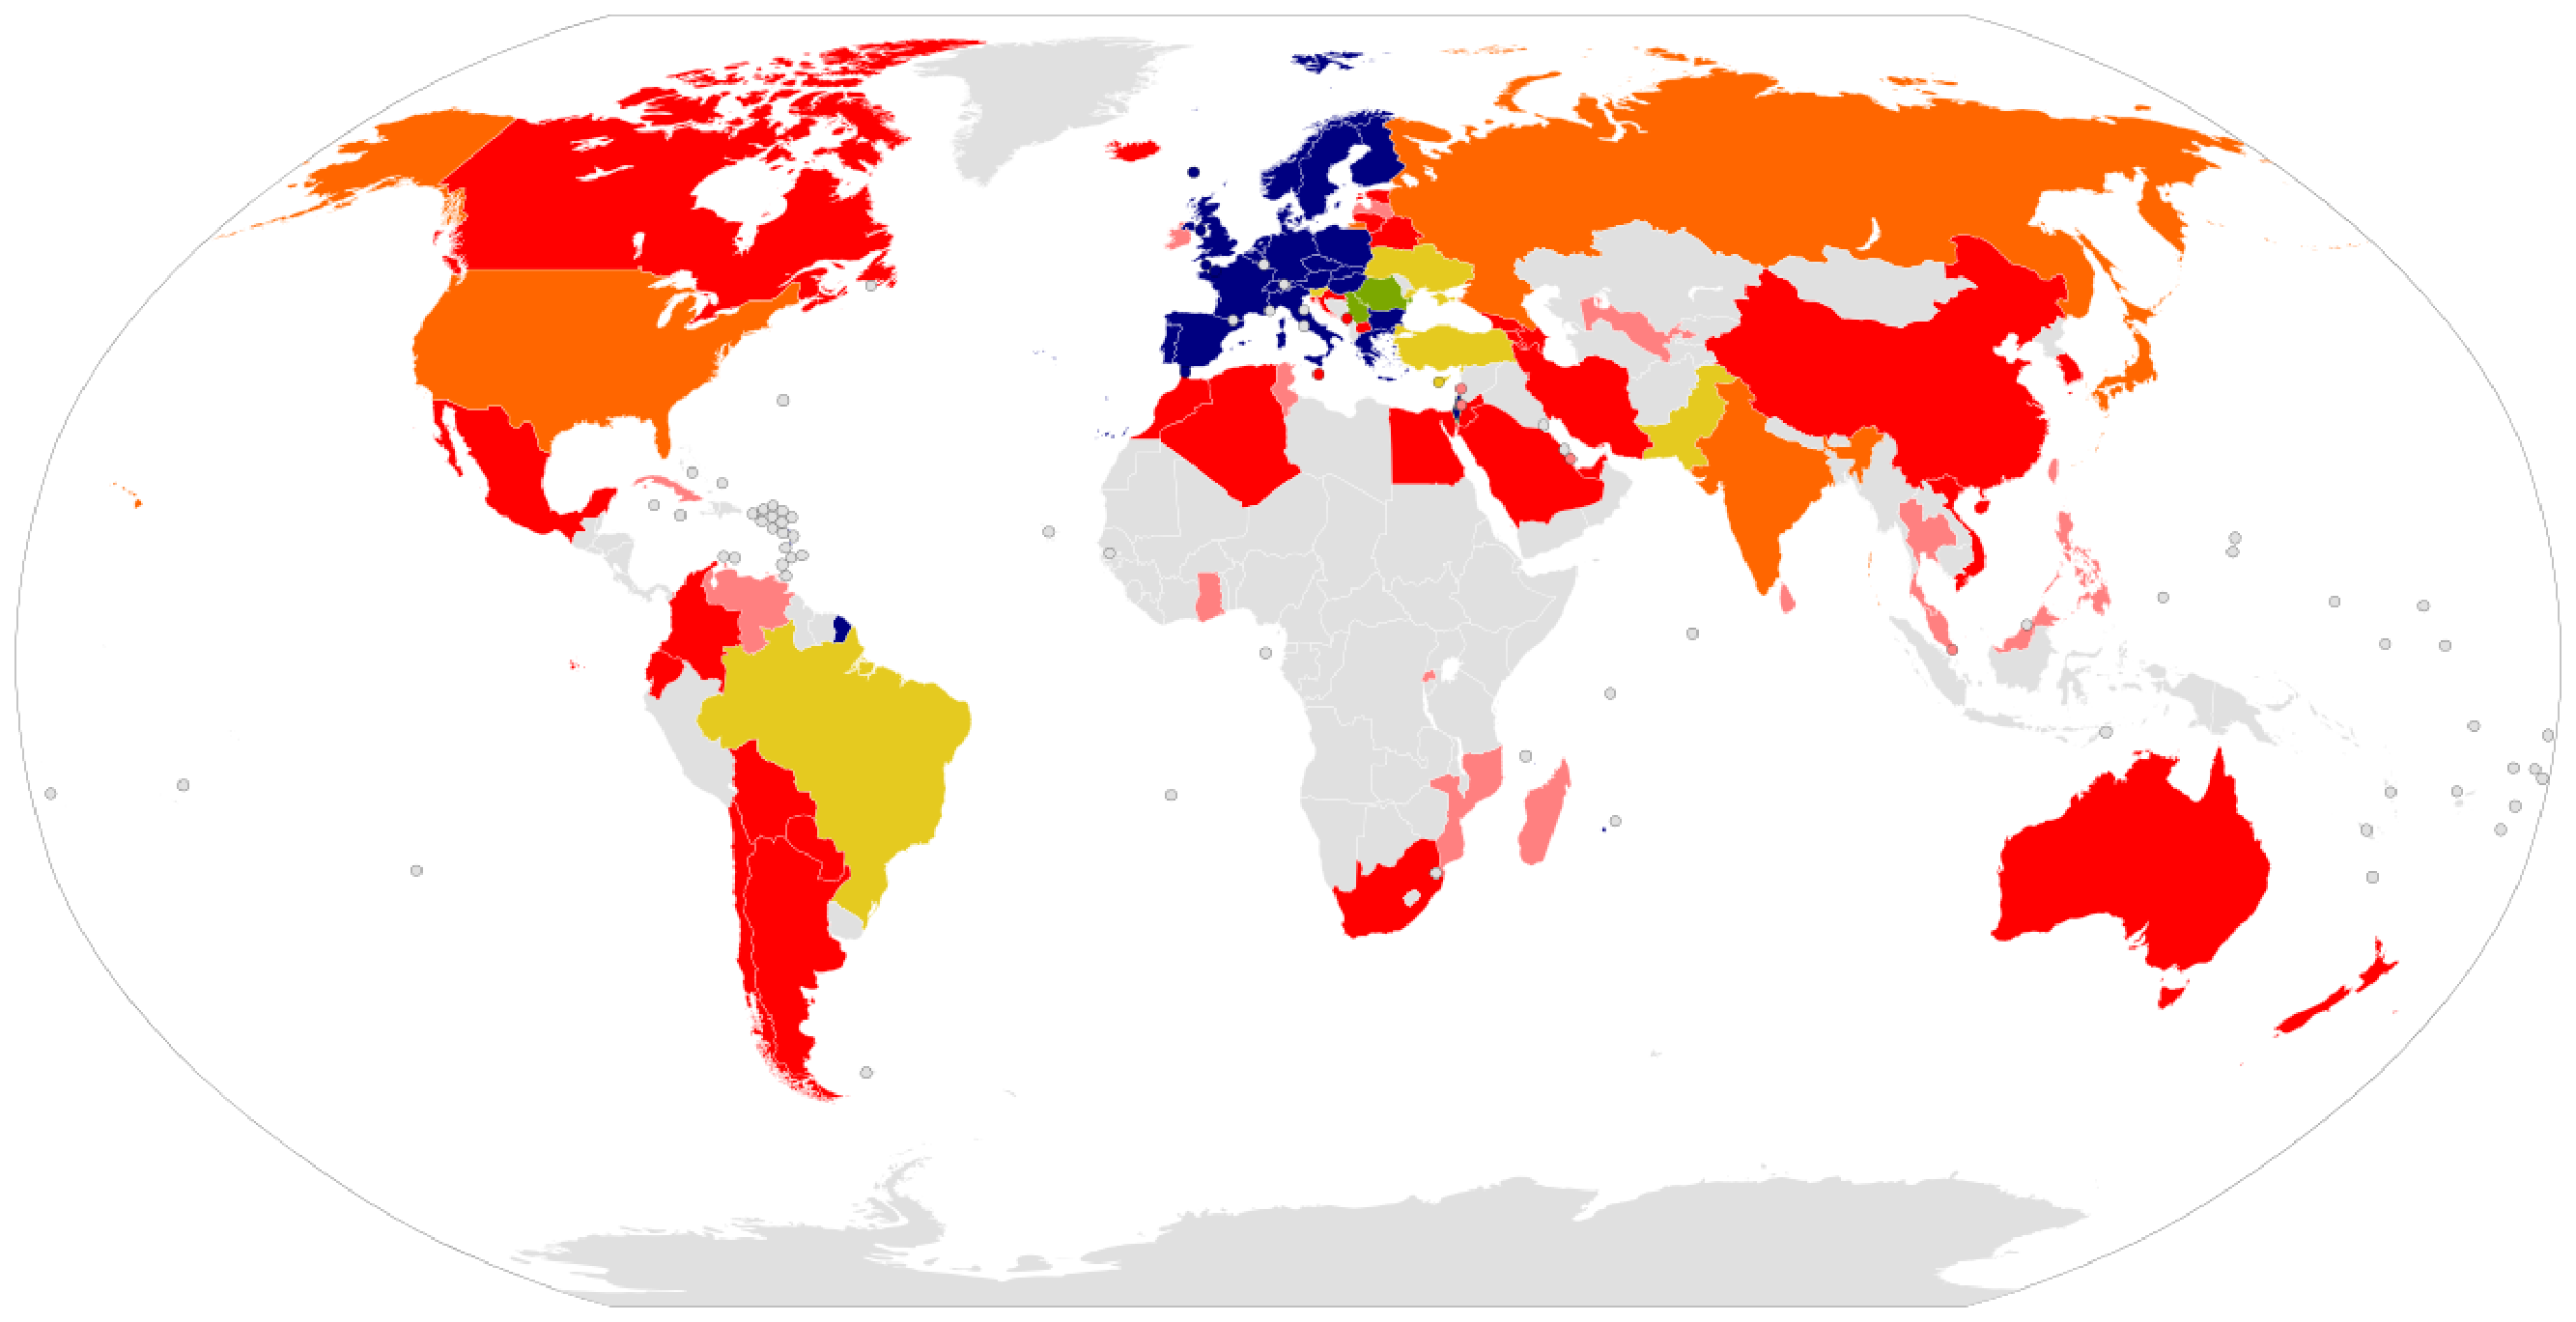
\includegraphics[width=0.70\textwidth]{figures/experiment/CERN_international_relations_map.pdf}
      \end{center}
\caption{Map of the international relations each country has with CERN~\cite{cern:map}.
Member states are in blue. States for who accession is in progress are in green.
States who have declared intent to join are in yellow. Observers are in red. States with
cooperation agreements are in orange. States with scientific contacts are in pink.
}
\label{fig:cernmembers}
\end{figure}


\section{LHC\label{sec:LHC}}
\subsection{Overview}
The LHC~\cite{cern-jinst-lhc} is a $pp$ accelerator that straddles the border between France and Switzerland. It was installed in a 27 km tunnel with diameter 3.7 m at an average depth of 100 m underground.
The position of this tunnel with respect to nearby political and geographical points of interest is 
shown in Figures~\ref{fig:lhc_mapwithcities} and \ref{fig:lhc_map_tuna}.
The tunnel was previously
used by the Large Electron-Positron Collider (LEP)~\cite{LEP_DR1979} from 1989 to 2000 for electron-positron collisions.

\begin{figure}[ht]
 \begin{center}
    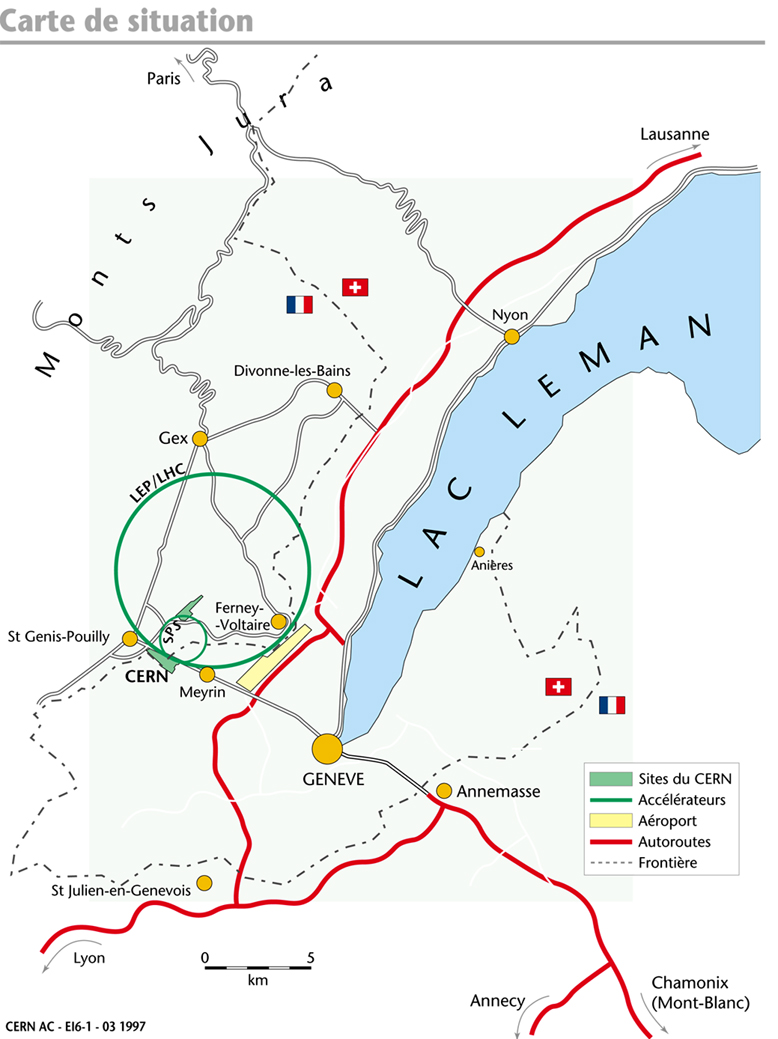
\includegraphics[width=0.70\textwidth]{figures/experiment/lhc-pho-1997-169.jpg}
      \end{center}
\caption{Map of the political and geographical highlights near the LHC~\cite{Dailler:842399}.}
\label{fig:lhc_mapwithcities}
\end{figure}

\begin{figure}[ht]
 \begin{center}
    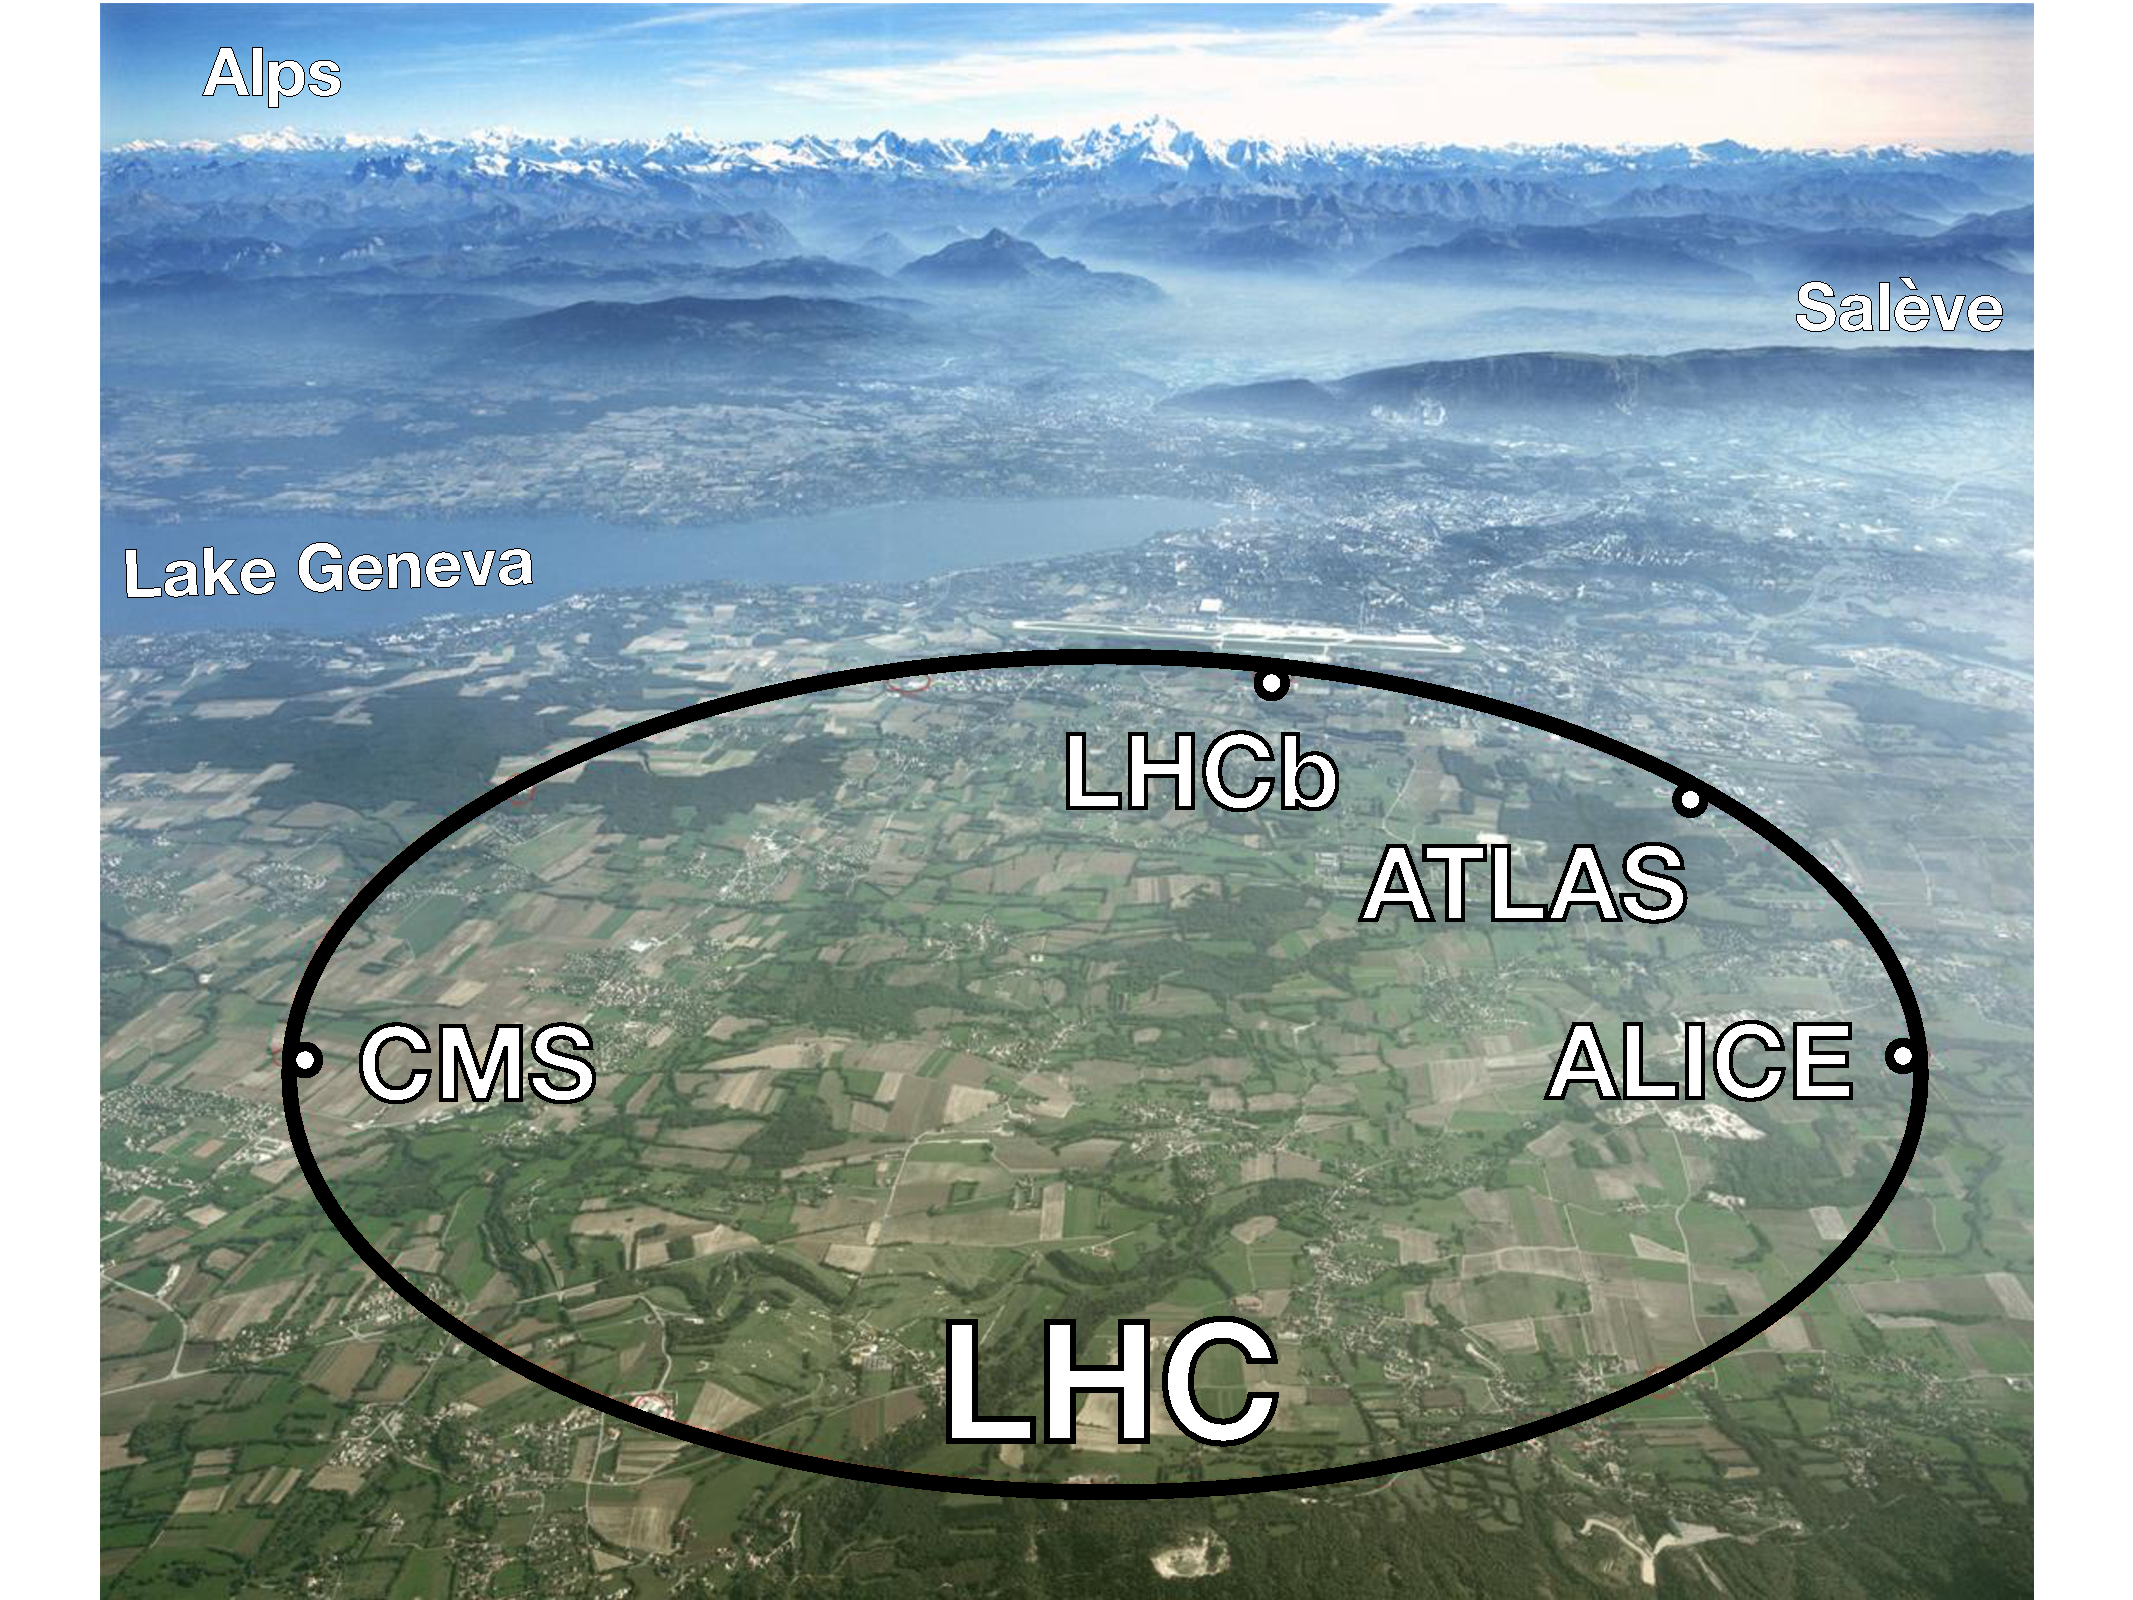
\includegraphics[width=0.90\textwidth]{figures/experiment/lhc-switzerland.pdf}
      \end{center}
\caption{Arial photo of the Geneva countryside with the LHC superimposed~\cite{Tuna:thesis}.}
\label{fig:lhc_map_tuna}
\end{figure}

The LHC is designed to accelerate protons or ions in two circular beam pipes, orbiting in opposite directions~\cite{cern-accelerators}. The pre-accelerators are described in Subsection~\ref{subsec:accelerators}, while the LHC
itself is described in Subsection~\ref{subsec:machine}
These beams are made to cross in four designated points of the accelerator and create collisions between
pairs of particles in opposite beams.
Each of these points is home to a large detector which measures the
products of these collisions, which are described in Subsection~\ref{subsec:detectors}.

\subsection{Accelerator Complex\label{subsec:accelerators}}

The path that a proton takes before entering a collision in the middle of CMS is shown in
Figure~\ref{fig:cern_accelerators}. Hydrogen gas is stripped of its electron and accelerated in
Linac2, a linear accelerator, to 50 MeV. Next are a series of three circular pre-accelerators that
increase the kinetic energy of the protons as well as collect the protons into discrete bunches.
These accelerators are the Proton Synchrotron Booster (PSB), the Proton Synchrotron (PS), and the
Super Proton Synchrotron (SPS), which increase the proton's energy to 1.4 GeV, 25 GeV, and 450 GeV,
respectively. 

\begin{figure}[ht]
 \begin{center}
    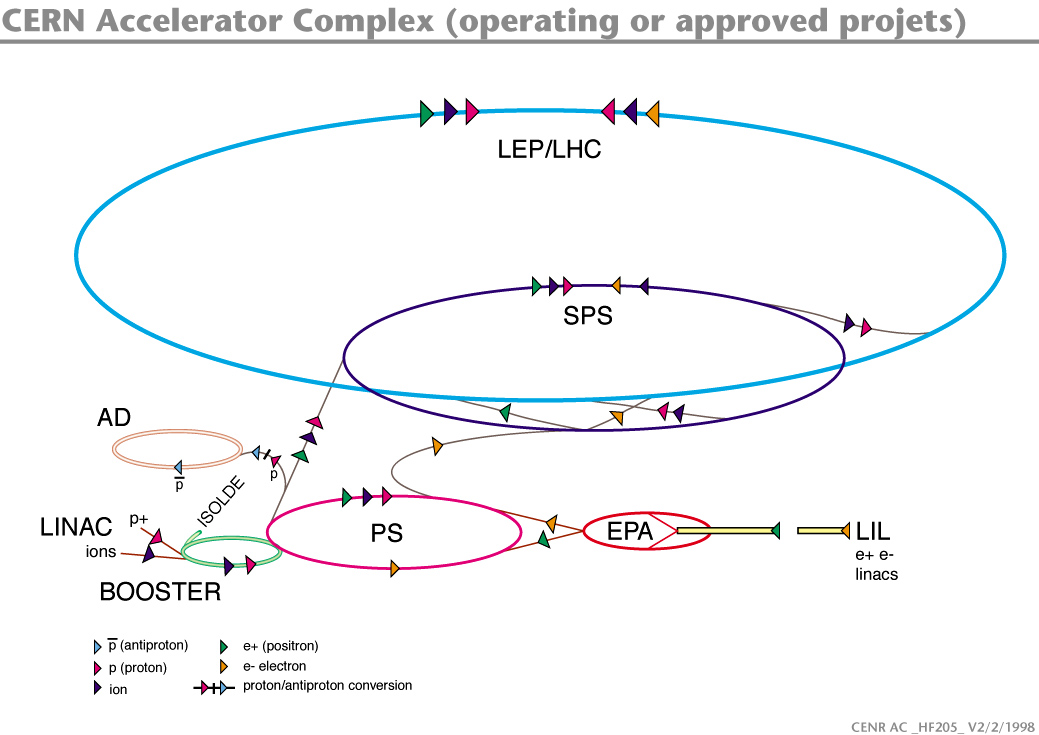
\includegraphics[width=0.90\textwidth]{figures/experiment/lhc-pho-1991-001.jpg}
      \end{center}
\caption{The flow of the CERN accelerator complex~\cite{Jean-Luc:841493}.}
\label{fig:cern_accelerators}
\end{figure}

After the SPS, the protons are injected into the LHC, where they are accelerated to up to 7 TeV.
The bunch structure is maintained during injection into the LHC, which is important for the timing
of the collisions inside the detectors. 

\subsection{The Machine\label{subsec:machine}}

The LHC is made up of 1232 dipole magnets divided by eight insertion points. A cross sectional view
of a dipole is shown in Figure~\ref{fig:lhc_dipole}. The purpose of the
dipoles, each of which has two holes for each beam, is to direct the proton beams on their circular
path. To keep these high energy particles on their path, each dipole produces a magnetic field
of 8.3 T using a superconductor cooled with liquid helium to 1.9 K, which allows for a current
of 12 kA. The length and mass of a dipole is 14 m and 35 tons, respectively.

\begin{figure}[ht]
 \begin{center}
    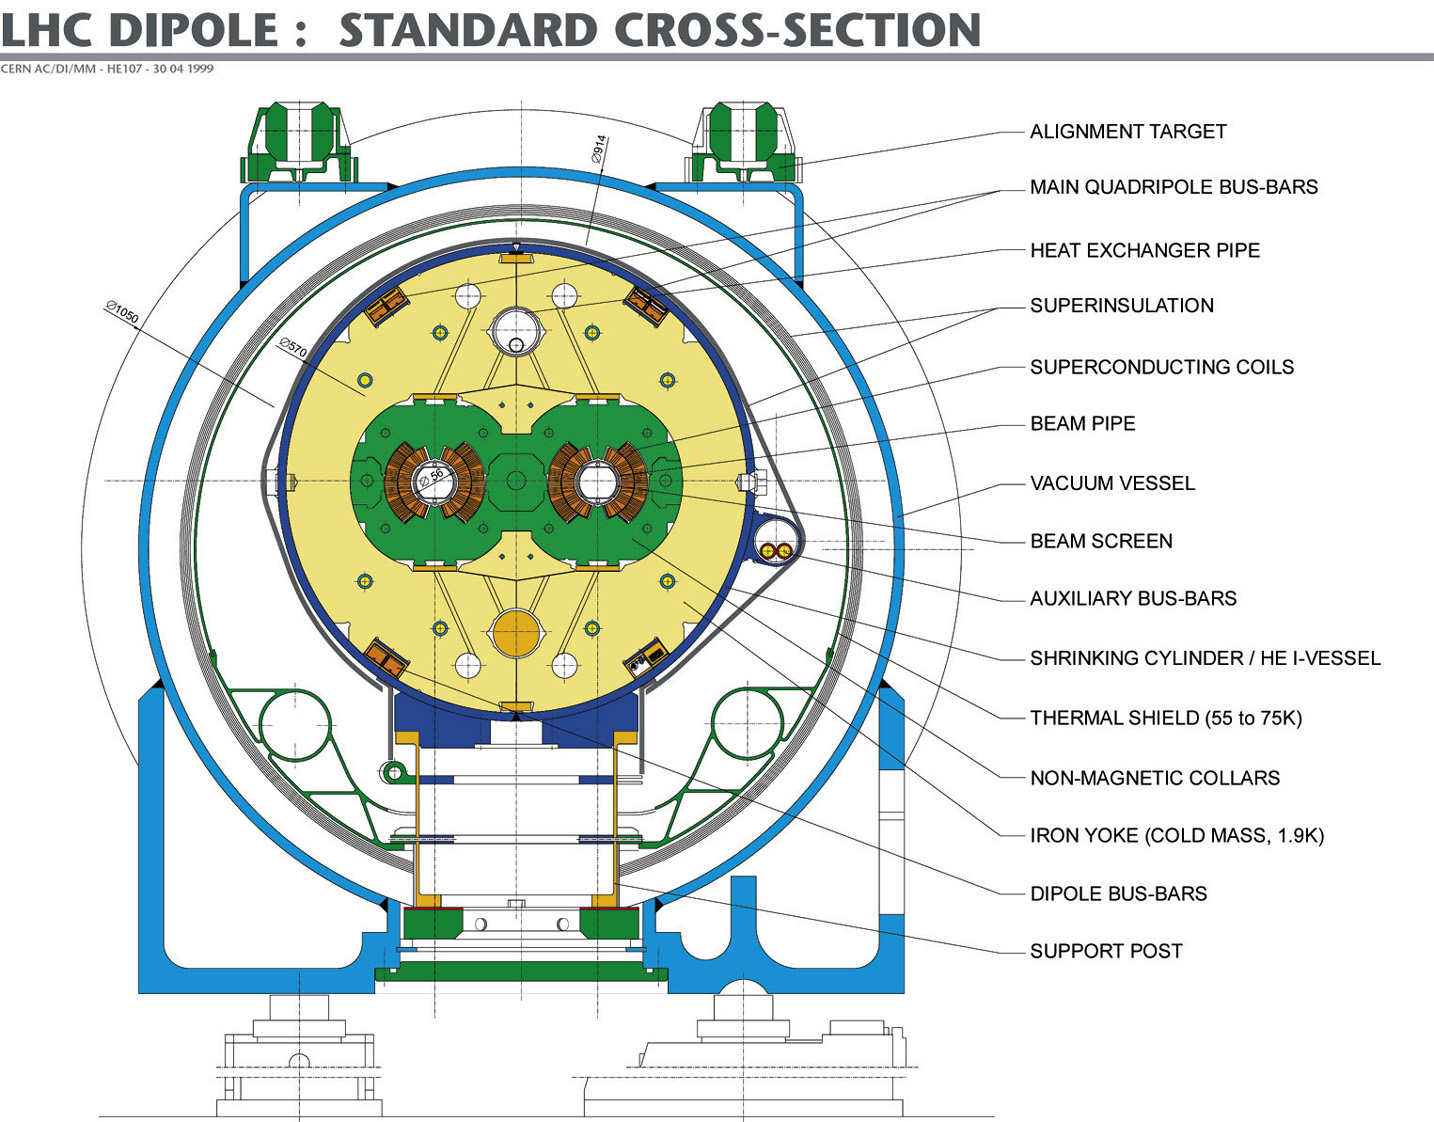
\includegraphics[width=0.90\textwidth]{figures/experiment/9906025_01.jpeg}
      \end{center}
\caption{Digram of a cross section of an LHC dipole~\cite{Team:40524}.}
\label{fig:lhc_dipole}
\end{figure}

Each insertion point serves a different purpose. Points 1, 2, 5, and 8 are the interaction points, where
the beams overlap to produce collisions. Point 4 contains the radio frequency cavity systems, which
provide acceleration to the particles in the direction of their motion. Points 3 and 7 contain beam
collimation systems. Point 6 contains beam dump systems for removing the beams from the LHC.

\subsection{Detectors on the LHC\label{subsec:detectors}}

The general purpose detectors on the LHC are A Toroidal LHC Apparatus (ATLAS)~\cite{cern-jinst-atlas}
and CMS, located at opposite sides of the ring at points 1 and 5, respectively. The physics
goals of these two experiements are generally the same: to search for and study the Higgs boson,
to study and improve our understanding of SM processes, and to search for BSM physics such as
SUSY or WED.

The Large Hadron Collider beauty detector (LHCb)~\cite{cern-jinst-lhcb}
is located at point 8 and is used
to study processes related to the bottom quark. A Large Ion Collider Experiment
(ALICE)~\cite{cern-jinst-alice} is located
at point 2 and is used to solely to study collisions when one or both beams contain lead ions. This
mode of operation of the LHC lasts about one to two months per year.

The relative positions of these four detectors on the LHC is shown in Figure~\ref{fig:lhc_detectors}.
Although the figure makes it appear that all the experiments are at the same depth, the LHC tunnel is
actually sloped at 1.5 degrees toward Lac Leman, causing the tunnel depth to vary between 50 and 150 m.

\begin{figure}[ht]
 \begin{center}
    \includegraphics[width=0.90\textwidth]{figures/experiment/9906026.jpg}
      \end{center}
\caption{Underground view of the LHC and the relative positions of the four detectors~\cite{Dailler:842399}.}
\label{fig:lhc_detectors}
\end{figure}

\subsection{2012 Running}

The principle physics result described in this work is an analysis of the data taken with the
CMS detector during the operation of the LHC in 2012. During this time, the center-of-mass energy
of the $pp$ collisions was $\sqrt{s} = 8$~TeV, whereas the design center-of-mass energy of
$\sqrt{s} = 14$~TeV will be acheived in future operation of the LHC. 

Of the $10^{11}$ protons in each bunch, only a small number of pairs of protons interact during
a bunch crossing inside CMS, where the beams are squeezed into a smaller transverse region. This number
varies from fill to fill and even within a fill due to conditions in the accelerator. The distribution
of the pileup during 2012 running is given in Figure~\ref{fig:pileup2012}, during which time the
average was 21.

\begin{figure}[ht]
 \begin{center}
    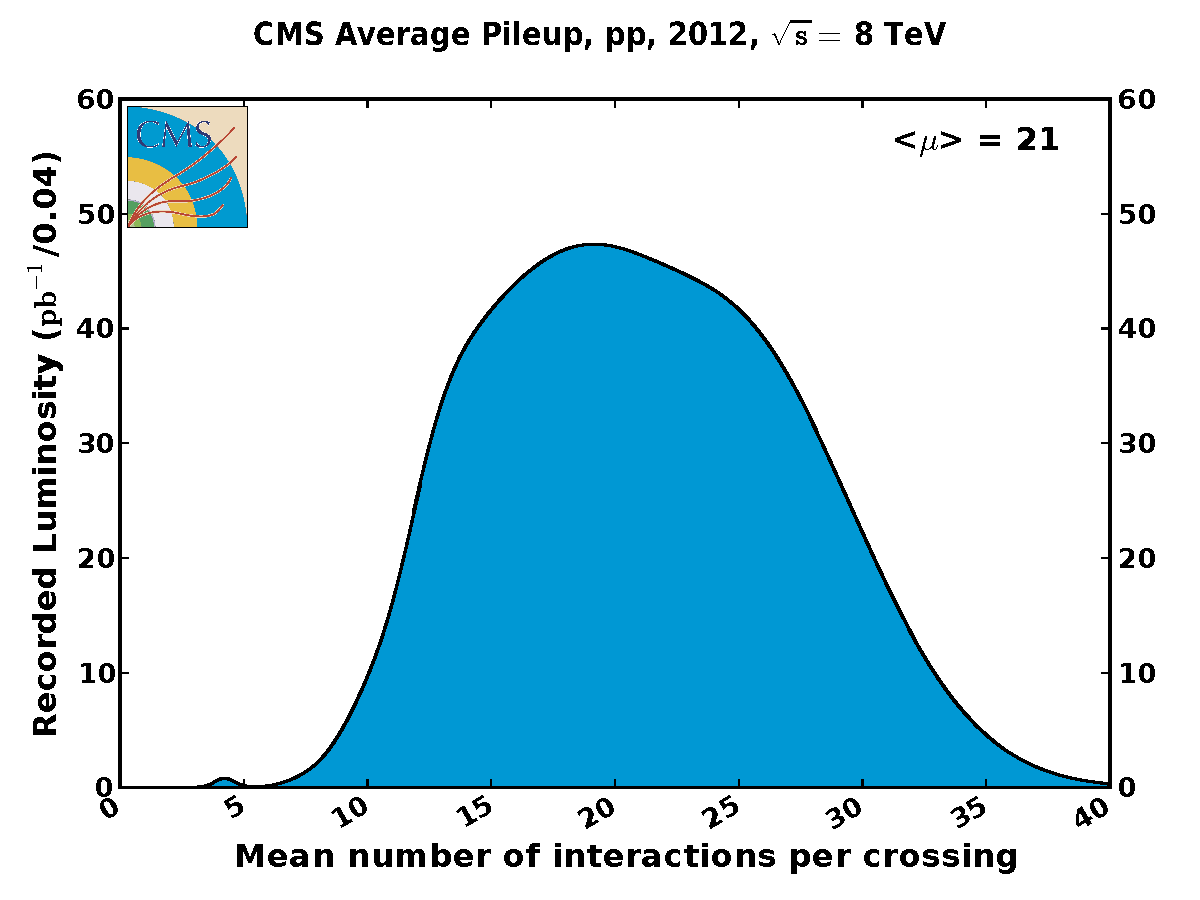
\includegraphics[width=0.90\textwidth]{figures/experiment/pileup_pp_2012.pdf}
      \end{center}
\caption{The average pileup in CMS during 2012~\cite{CMS:lumi}.}
\label{fig:pileup2012}
\end{figure}

The total integrated luminosity delivered to CMS during this time was $23.3$~fb~$^{-1}$.
The evolution of the integrated luminosity delivered to and recorded by CMS is shown in
Figrure~\ref{fig:integratedlumi2012}. The delivered integrated luminosity is the amount of
collisions delivered by the LHC to CMS, and ideally CMS would be able to same all of these collisions.
Due to limitations of the data acquisition chain or availability of each subsystem, discussed in
Sections~\ref{sec:trigger} and \ref{sec:CMS}, respectively, the amount recorded
is slightly less than the delivered. In 2012, the total recorded luminosity was $21.8$~fb~$^{-1}$.

\begin{figure}[ht]
 \begin{center}
    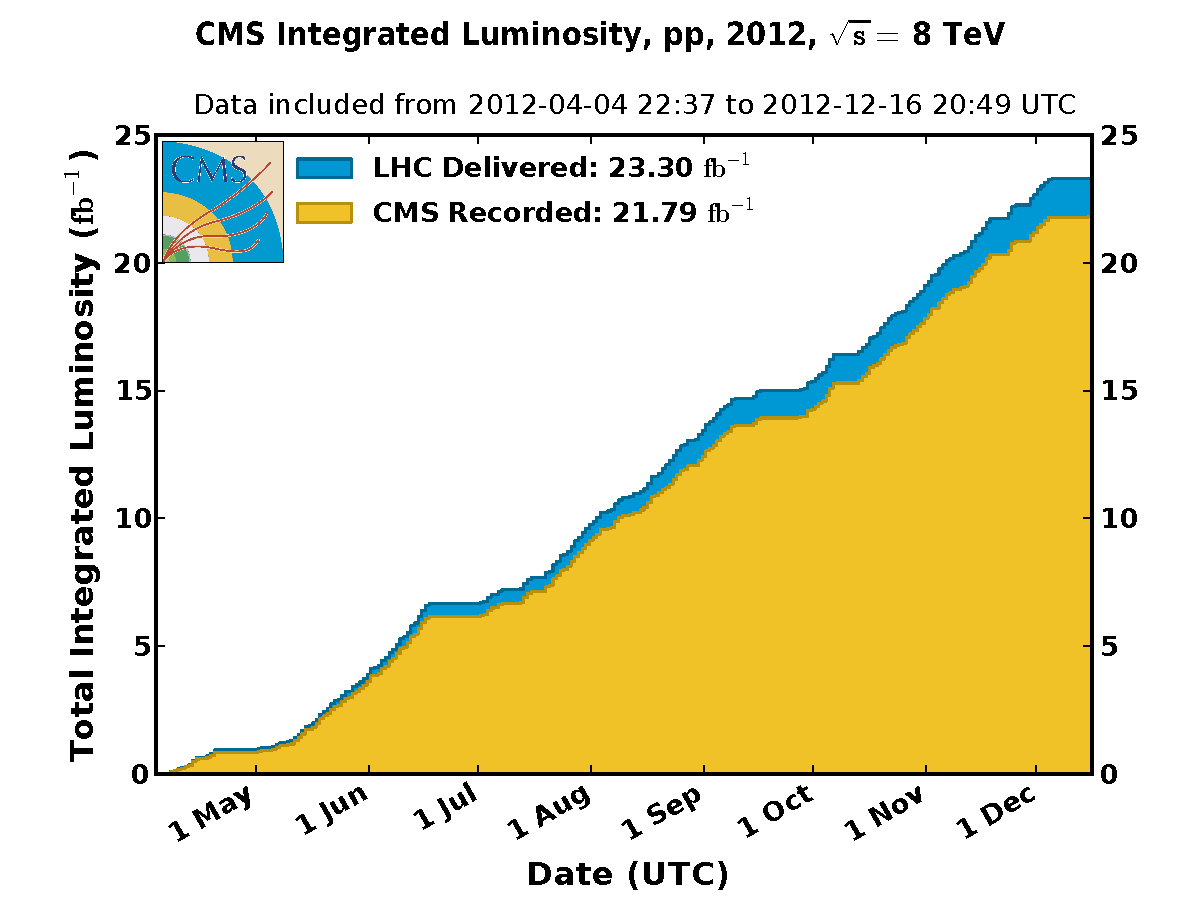
\includegraphics[width=0.90\textwidth]{figures/experiment/int_lumi_per_day_cumulative_pp_2012.pdf}
      \end{center}
\caption{The integrated luminosity of $pp$ collisions in CMS during 2012~\cite{CMS:lumi}.}
\label{fig:integratedlumi2012}
\end{figure}

The LHC delivered $pp$ collisions in 2010 and 2011 at $\sqrt{s} = 7$~TeV,
and these were also recorded by CMS.
Figure~\ref{fig:intlumi101112} shows the total luminosity delivered to CMS in each of these years.
Although the $6.1$~fb~$^{-1}$ of 2011 data is used in many measurements of the Higgs boson and
other SM processes, this analysis of diHiggs production pertains principally to 8~TeV data.

\begin{figure}[ht]
 \begin{center}
    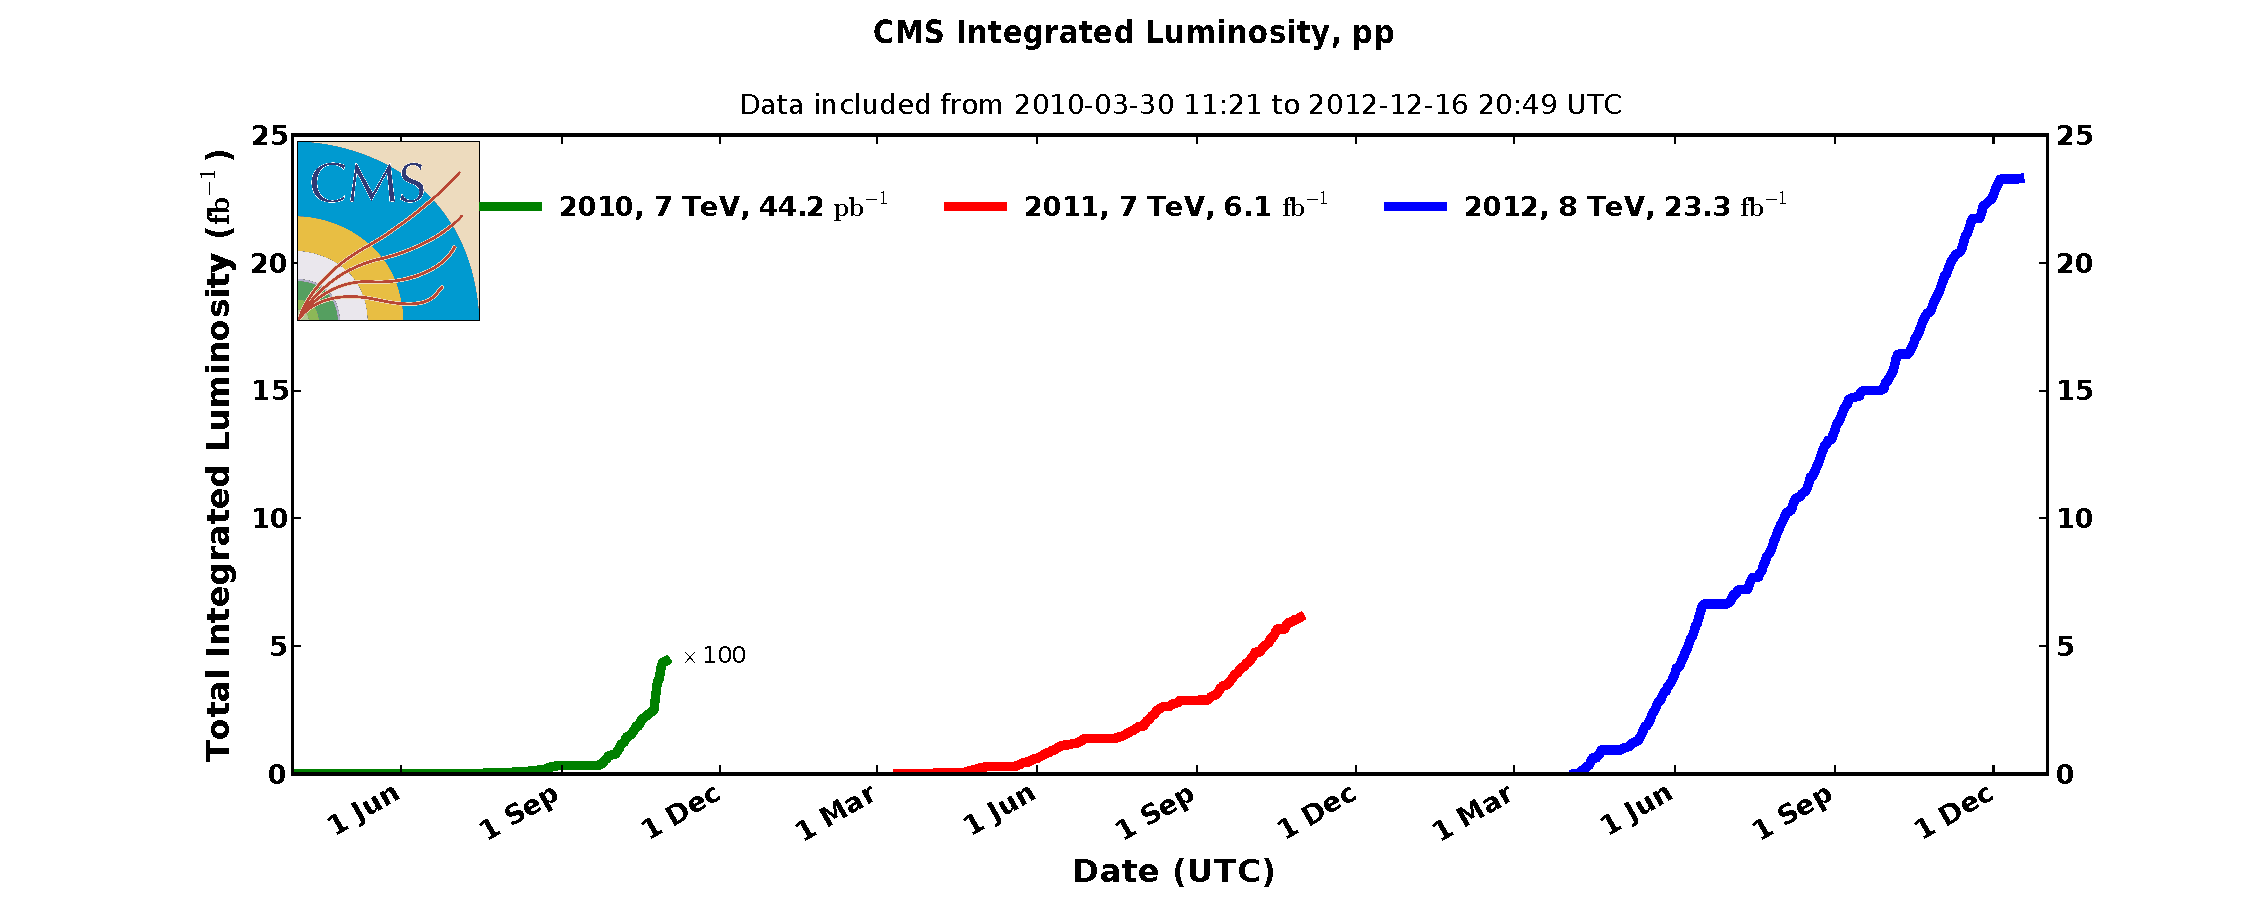
\includegraphics[width=0.90\textwidth]{figures/experiment/int_lumi_cumulative_pp_1.pdf}
      \end{center}
\caption{The integrated luminosity of $pp$ collisions in CMS from 2010 to 2012~\cite{CMS:lumi}.}
\label{fig:intlumi101112}
\end{figure}

%Design lumi $\mathcal{L} = \pow{10,34}$~cm$-2$s$-1$. 

\section{CMS\label{sec:CMS}}

CMS is one of the two general purpose detectors on the LHC. It was built in part
to search for the Higgs boson on the range of masses not already excluded by previous experiments
and by theory, as already discussed in Section~\ref{sec:discovery}. Other physics goals include
the study of aspects of the SM, such as the top quark mass, and the search for BSM physics, such
as supersymmetry, extra dimensions, and dark matter, as already discussed in
Section~\ref{sec:SMshortcomings}.

The CMS coordinate system is defined with the origin at the center of the detector. The $z$-axis
of this coordinate system points in the direction that the counterclockwise beam takes at this origin.
The transverse plane is perpendicular to this axis, with the $x$-axis pointing to the center of the
circle made by the LHC and the $y$-axis pointing vertically upward. The azimuthal angle $\phi$ gives
the angle in the transverse plane as measured counterclockwise from the $x$-axis, and the polar angle
$\theta$ is measured from the $z$-axis. In CMS, as the case with other collider experiments,
a Lorentz-invariant pseudorapidity $\eta$ is used in place of the polar angle. It is given by

\begin{equation}
\eta = -\log\left(\frac{\theta}{2}\right) .
\end{equation}

The central feature of CMS is its superconducting solenoid magnet~\cite{cms:solenoid}.
At 12.5~m long and with an internal diameter of 6~m, it is the world's largest superconducting magnet.
The superconducting material is niobium-titanium, which is cooled to 4~K and provided with a current
of 18~kA.
It is centered on the IP and provides a uniform magnetic field inside its volume of 3.8~T.
Outside of the solenoid, an iron return yoke returns the magnetic field which escapes the ends
of the cylinder. The field strength in this region is a uniform 2 T.

CMS is described in detail in \cite{Chatrchyan:2008zzk} and \cite{Bayatian:922757}.
Here an overview of each of the subsystems
is provided, starting from the closest to the main interation point (IP) and proceeding
radially outward. Figure~\ref{fig:CMS_side} gives relative position and sizes of each of the
subsystems.
Subsection~\ref{subsec:tracker} covers the silicon tracker. Subsection~\ref{subsec:ecal} covers the
electromagnetic calorimeter (ECAL). Subsection~\ref{subsec:hcal} covers the hadronic calorimeter
(HCAL). After the HCAL is the solenoidal magnet, which, although not directly contributing to the
description of an event, is necessary for measuring the energy of charged particles through
the reconstruction of their tracks. Subsection~\ref{subsec:muonsystem} covers the muon system.

\begin{figure}[ht]
 \begin{center}
   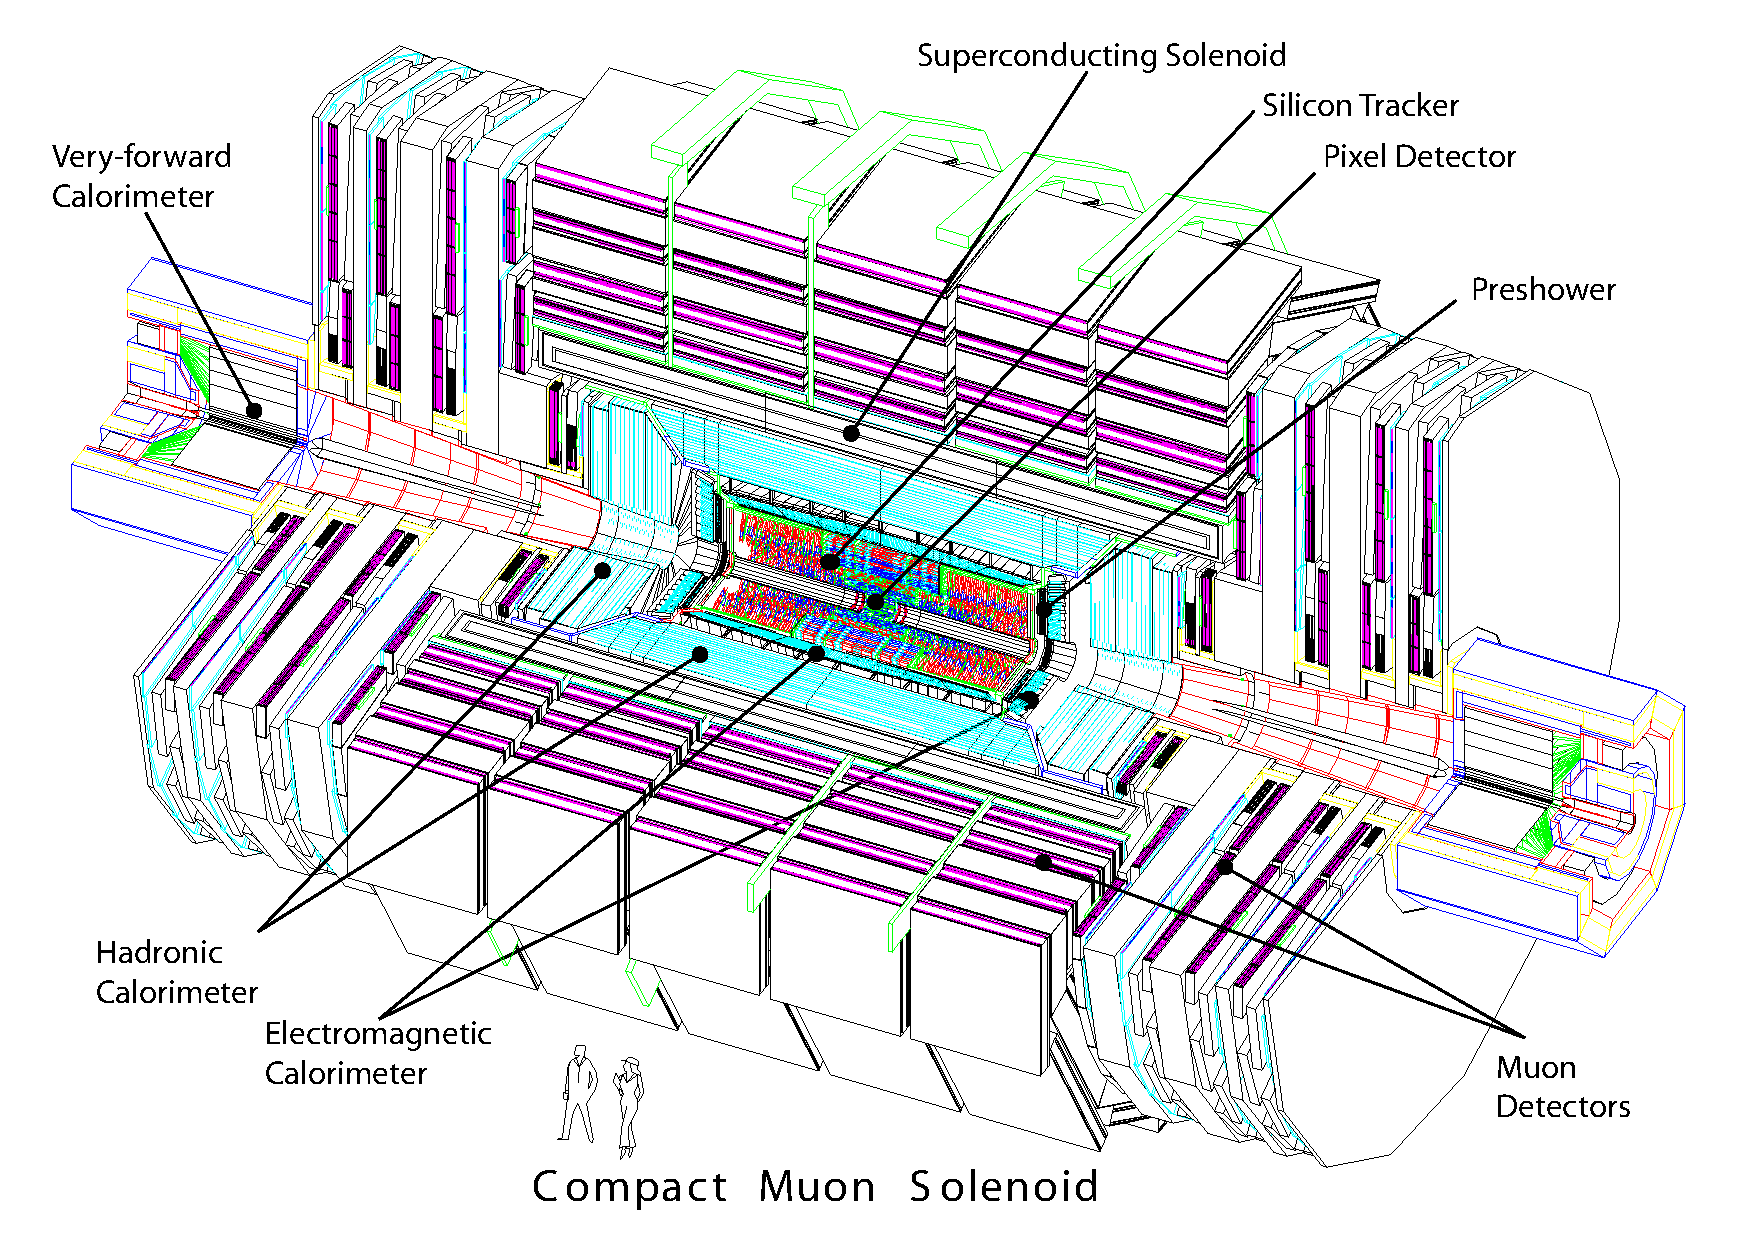
\includegraphics[width=0.90\textwidth]{figures/experiment/cms_complete_labelled.pdf}
      \end{center}
\caption{The CMS detector, with two people to give a sense of scale~\cite{Collaboration:1433717}.}
\label{fig:CMS_side}
\end{figure}

\subsection{Silicon Tracker\label{subsec:tracker}}

The silicon tracker~\cite{Karimaki:368412} is responsible for measuring the positions of charged particles as they propogate from the IP.
The goal is reconstruct the paths of these charged particles by recording their position
in successive layers of silicon. When coupled with the strong magnetic field provided by the solenoid
magnet, the charged particles have a curled trajectory, the radius of which is related directly
to the particles transverse momentum $p_{\rm T}$. A stronger field means better momentum resolution.

The choice of silicon technology is imperative to achieve this goal.When a charged particle passes throught the material, electrons are liberated from the atoms of the semiconductor, and a bias voltage
allows for the collection of this free electron and electon hole. If the charged collected during
a time window exceeds a certain value, a hit is registered, and the hits from successive layers
are reconstructed offline for particle identification and momentum measurements.
Section~\ref{sec:PF} discusses the Particle Flow algorithm used for performing this identification.

The tracker itself occupies a volume
of length 5.4~m and radius 1.1~m and can cover detection up to $|\eta| < 2.5$. It is divided into
the pixel detector and strip detector, both of which are divided into barrel regions, or those
where the layers are parallel to the $z$-axis, and endcap regions, or those where the layers
are parallel to the transverse plane.

The pixel detector has three layers in the barrel region
and two layers on either end in the endcap region, in total making up 66 million channels of size
$100 \mu m \times 150 \mu m$. The strip detector surrounds the pixel detector and adds an additional
10 layers in the barrel and 12 layers in each endcap. The silicon strips vary in size from
$10 cm \times 80 \mu m$ to $25 cm \times 180 \mu m$ and in orientation, either parallel or perpendicular
to the $z$-axis.

\subsection{Electromagnetic Calorimeter\label{subsec:ecal}}

The ECAL~\cite{ecaltdr} is a calorimeter that focuses on measuring the energy of electromatic showers.
It, like the tracker, is divided into barrel and endcap regions, and provides coverage up to
$|\eta| < 3.0$.
It accomplishes this by employing 75 thousand lead tungstate crystals of size
$25 mm \times 25 mm \times 230 mm$ in the barrel or $30 mm \times 30 mm \times 220 mm$ in the endcap.
The ECAL is 25 radiation lengths long, a relatively large number that is exploited in
particle identification. Electrons and photons are stopped by having their energy dissipated
through many cascades, electrons through bremsstrahlung and photons through pair production.
Hadrons and muons, also interacting electromagnetically, deposit some energy
but are able to pass through to the HCAL due to, in part, their larger masses. The energy resolution
provided by the ECAL is

\begin{equation}
\frac{\sigma(E)}{E} = \frac{0.028}{\sqrt{E/\textrm{GeV}}} \oplus \frac{0.12}{E/\textrm{GeV}} \oplus 0.3\% .
\end{equation}

\subsection{Hadronic Calorimeter\label{subsec:hcal}}

The last subsystem within the volume of the solenoid magnet is HCAL~\cite{hcaltdr}.
The subsystem has barrel and endcap divisions similar to ECAL which covers up to $|\eta| < 3.0$.
These components are made of plastic scintillator and brass absorber which form 3700 towers. The
towers vary in coverage based on their placement, where the most central towers span
$\Delta\eta \times \Delta\phi = 0.087 \times 0.087$. The purpose of this subsystem is to
measure the energy of hadrons, which usually appear in columnated sprays called jets $j$. In addition
to energy and position measurement, nearly all hadrons are stopped and absorbed due to the
high density of large material budget of brass. There is an additional component of the HCAL
in the barrel region immediately outside of the magnet whose purpose is to serve as another
layer of absorbtion for any hadrons that make it through preceeding layers.

A final component covers pseudorapidities $3.0 < |\eta|< 5.0$. In this region, the damage from
radiation is especially high, so here a stell and quartz-fibre \v{C}erenkov calorimeter is used.
This region provides 860 such towers.

The energy resolution is improved from the incorporation of information from other subsystems via
the Particle Flow algorithm, discussed in Section~\ref{sec:PF}.
The resolution is about 15\% for jets of interest to this analysis, those which are central and
have sufficient high $p_{\rm T}$. Section~\ref{sec:jets} discusses these requirements.

Figure~\ref{fig:subsystems_inner} shows a quadrant of the inner subsystems of CMS. This gives
a scale of the relative positions and sizes of the tracker, ECAL,
and most of HCAL with respect to eachother and the IP. Missing from the HCAL are the 
HCAL Forward (HF) in the very forward region and the HCAL outer barrel (HO) just to the outside of
the magnet.

\begin{figure}[ht]
 \begin{center}
   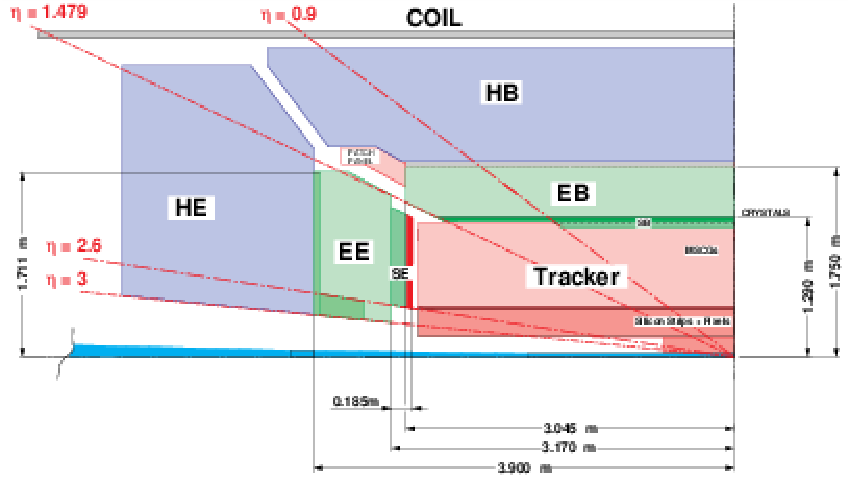
\includegraphics[width=0.90\textwidth]{figures/experiment/subsystems_inner.pdf}
      \end{center}
\caption{A schematic of one quarter of the inner CMS subsystems~\cite{ecaltdr}.
All components of the tracker are in red. The ECAL barrel (EB) and ECAL endcap (EE) are in blue.
The HCAL barrel (HB) and HCAL endcap (HE) are in green. Coil refers to the superconducting solenoid.
Dimensions and lines of constant $\eta$ from the IP are superimposed.}
\label{fig:subsystems_inner}
\end{figure}


\subsection{Muon System\label{subsec:muonsystem}}

The muon system~\cite{muontdr} is the subsystem furthest from the IP and measures the positions
of muons through detection planes exploiting three different technologies:
drift tubes (DT), resistive plate chambers (RPC), and cathode strip chambers (CSC).
Together these components provide muon coverage up to $|\eta|< 2.4$.
The DTs, located in the barrel, are gas tubes with a wires for collecting electrons liberated
by a transvering muon. The RPCs, partially coveraging both barrel and endcap regions, consist
of two parallel plates of opposite bias separated by a gas medium. The CSCs, covering the endcap region,
consist of layers of anode, separated by layers of cathode wires oriented perpendicularly, all
within a gas volume. Figure~\ref{fig:muonsystem} shows the relative position of these three components with respect to eachother and the subsystems inside the solenoid.

The hits of the muon system are matched with hits from the tracker to form a single track and
improve momentum resolution. Unlike other charged particles, which register significant activity in
one or both calorimeters, the energy measurement of muons is based purely on their tracks. This means
that the resolution worsens for higher energy muons as their tracks are less and less curled by
the magnetic field.


\begin{figure}[ht]
 \begin{center}
   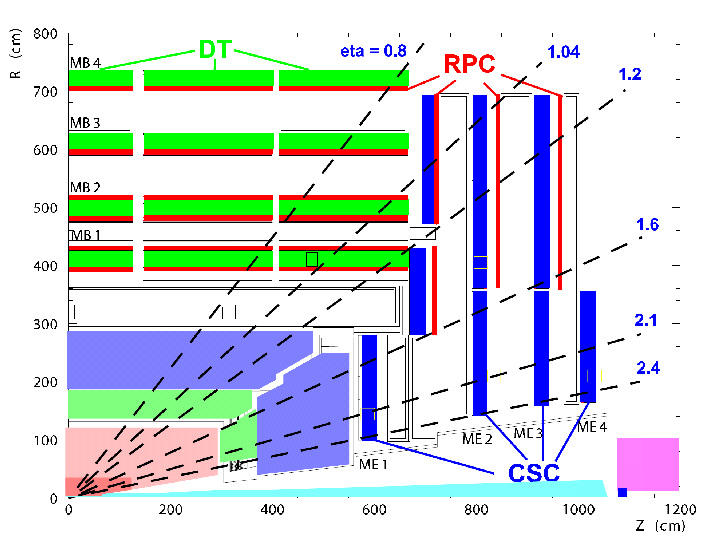
\includegraphics[width=0.90\textwidth]{figures/experiment/muons.pdf}
      \end{center}
\caption{A schematic of one quarter of the muon systems~\cite{Chatrchyan:2008zzk}.
Lines of constant $\eta$ from the IP are superimposed.}
\label{fig:muonsystem}
\end{figure}


